\chapter{Đồ thị có hướng}

Trong chương này, chúng ta tập trung vào hai loại đồ thị có hướng:
\begin{itemize}
\item \key{Đồ thị không có chu trình (Acyclic graphs)}:
Không có chu trình nào trong đồ thị,
vì vậy không có đường đi từ bất kỳ nút nào đến chính nó\footnote{Đồ thị có hướng không chu trình đôi khi được gọi là DAGs.}.
\item \key{Đồ thị kế tiếp (Successor graphs)}:
Bán bậc ngoài của mỗi nút là 1,
vì vậy mỗi nút có một nút kế tiếp duy nhất.
\end{itemize}
Hóa ra trong cả hai trường hợp,
chúng ta có thể thiết kế các thuật toán hiệu quả dựa trên
các thuộc tính đặc biệt của các đồ thị này.

\section{Sắp xếp tô pô (Topological sorting)}

\index{sắp xếp tô pô}
\index{chu trình}

Một \key{sắp xếp tô pô} là một cách sắp xếp thứ tự
các nút của một đồ thị có hướng
sao cho nếu có một đường đi từ nút $a$ đến nút $b$,
thì nút $a$ xuất hiện trước nút $b$ trong thứ tự đó.
Ví dụ, đối với đồ thị
\begin{center}
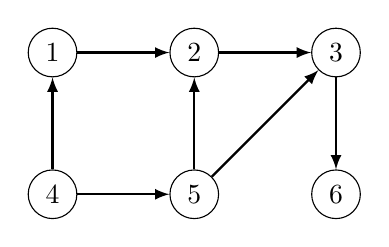
\begin{tikzpicture}[scale=0.9]
\node[draw, circle] (1) at (1,5) {$1$};
\node[draw, circle] (2) at (3,5) {$2$};
\node[draw, circle] (3) at (5,5) {$3$};
\node[draw, circle] (4) at (1,3) {$4$};
\node[draw, circle] (5) at (3,3) {$5$};
\node[draw, circle] (6) at (5,3) {$6$};

\path[draw,thick,->,>=latex] (1) -- (2);
\path[draw,thick,->,>=latex] (2) -- (3);
\path[draw,thick,->,>=latex] (4) -- (1);
\path[draw,thick,->,>=latex] (4) -- (5);
\path[draw,thick,->,>=latex] (5) -- (2);
\path[draw,thick,->,>=latex] (5) -- (3);
\path[draw,thick,->,>=latex] (3) -- (6);
\end{tikzpicture}
\end{center}
một cách sắp xếp tô pô là
$[4,1,5,2,3,6]$:
\begin{center}
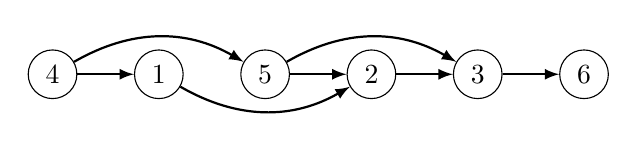
\begin{tikzpicture}[scale=0.9]
\node[draw, circle] (1) at (-6,0) {$1$};
\node[draw, circle] (2) at (-3,0) {$2$};
\node[draw, circle] (3) at (-1.5,0) {$3$};
\node[draw, circle] (4) at (-7.5,0) {$4$};
\node[draw, circle] (5) at (-4.5,0) {$5$};
\node[draw, circle] (6) at (-0,0) {$6$};

\path[draw,thick,->,>=latex] (1) edge [bend right=30] (2);
\path[draw,thick,->,>=latex] (2) -- (3);
\path[draw,thick,->,>=latex] (4) -- (1);
\path[draw,thick,->,>=latex] (4) edge [bend left=30] (5);
\path[draw,thick,->,>=latex] (5) -- (2);
\path[draw,thick,->,>=latex] (5) edge [bend left=30]  (3);
\path[draw,thick,->,>=latex] (3) -- (6);
\end{tikzpicture}
\end{center}

Một đồ thị không có chu trình luôn có một cách sắp xếp tô pô.
Tuy nhiên, nếu đồ thị chứa một chu trình,
thì không thể tạo thành một sắp xếp tô pô,
bởi vì không có nút nào của chu trình có thể xuất hiện
trước các nút khác của chu trình trong thứ tự đó.
Hóa ra, tìm kiếm theo chiều sâu (depth-first search) có thể được sử dụng
để vừa kiểm tra xem một đồ thị có hướng có chứa chu trình hay không
và, nếu nó không chứa chu trình, để xây dựng một sắp xếp tô pô.

\subsubsection{Thuật toán}

Ý tưởng là duyệt qua các nút của đồ thị
và luôn bắt đầu một tìm kiếm theo chiều sâu tại nút hiện tại
nếu nó chưa được xử lý.
Trong quá trình tìm kiếm, các nút có ba trạng thái khả dĩ:

\begin{itemize}
\item trạng thái 0: nút chưa được xử lý (màu trắng)
\item trạng thái 1: nút đang được xử lý (màu xám nhạt)
\item trạng thái 2: nút đã được xử lý (màu xám đậm)
\end{itemize}

Ban đầu, trạng thái của mỗi nút là 0.
Khi một tìm kiếm đến một nút lần đầu tiên,
trạng thái của nó trở thành 1.
Cuối cùng, sau khi tất cả các nút kế tiếp của nút đó đã
được xử lý, trạng thái của nó trở thành 2.

Nếu đồ thị chứa một chu trình, chúng ta sẽ phát hiện ra điều này
trong quá trình tìm kiếm, bởi vì sớm hay muộn
chúng ta sẽ đến một nút có trạng thái là 1.
Trong trường hợp này, không thể xây dựng một sắp xếp tô pô.

Nếu đồ thị không chứa chu trình, chúng ta có thể xây dựng
một sắp xếp tô pô bằng cách
thêm mỗi nút vào một danh sách khi trạng thái của nút đó trở thành 2.
Danh sách này theo thứ tự ngược lại là một sắp xếp tô pô.

\subsubsection{Ví dụ 1}

Trong đồ thị ví dụ, việc tìm kiếm đầu tiên tiến hành
từ nút 1 đến nút 6:

\begin{center}
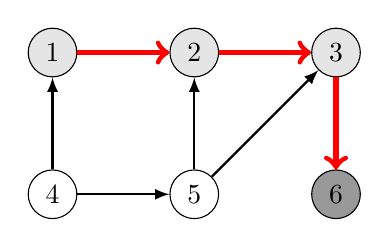
\begin{tikzpicture}[scale=0.9]
\node[draw, circle,fill=gray!20] (1) at (1,5) {$1$};
\node[draw, circle,fill=gray!20] (2) at (3,5) {$2$};
\node[draw, circle,fill=gray!20] (3) at (5,5) {$3$};
\node[draw, circle] (4) at (1,3) {$4$};
\node[draw, circle] (5) at (3,3) {$5$};
\node[draw, circle,fill=gray!80] (6) at (5,3) {$6$};

\path[draw,thick,->,>=latex] (4) -- (1);
\path[draw,thick,->,>=latex] (4) -- (5);
\path[draw,thick,->,>=latex] (5) -- (2);
\path[draw,thick,->,>=latex] (5) -- (3);
%\path[draw,thick,->,>=latex] (3) -- (6);

\path[draw=red,thick,->,line width=2pt] (1) -- (2);
\path[draw=red,thick,->,line width=2pt] (2) -- (3);
\path[draw=red,thick,->,line width=2pt] (3) -- (6);
\end{tikzpicture}
\end{center}

Bây giờ nút 6 đã được xử lý, vì vậy nó được thêm vào danh sách.
Sau đó, các nút 3, 2 và 1 cũng được thêm vào danh sách:

\begin{center}
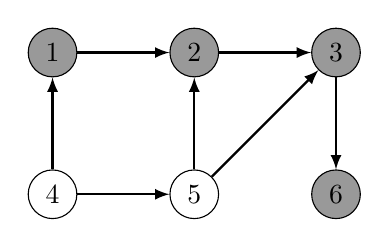
\begin{tikzpicture}[scale=0.9]
\node[draw, circle,fill=gray!80] (1) at (1,5) {$1$};
\node[draw, circle,fill=gray!80] (2) at (3,5) {$2$};
\node[draw, circle,fill=gray!80] (3) at (5,5) {$3$};
\node[draw, circle] (4) at (1,3) {$4$};
\node[draw, circle] (5) at (3,3) {$5$};
\node[draw, circle,fill=gray!80] (6) at (5,3) {$6$};

\path[draw,thick,->,>=latex] (1) -- (2);
\path[draw,thick,->,>=latex] (2) -- (3);
\path[draw,thick,->,>=latex] (4) -- (1);
\path[draw,thick,->,>=latex] (4) -- (5);
\path[draw,thick,->,>=latex] (5) -- (2);
\path[draw,thick,->,>=latex] (5) -- (3);
\path[draw,thick,->,>=latex] (3) -- (6);
\end{tikzpicture}
\end{center}

Tại thời điểm này, danh sách là $[6,3,2,1]$.
Việc tìm kiếm tiếp theo bắt đầu tại nút 4:

\begin{center}
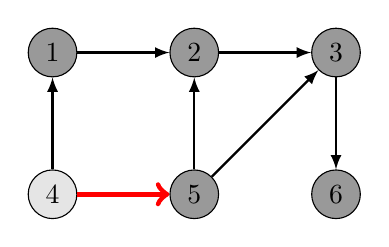
\begin{tikzpicture}[scale=0.9]
\node[draw, circle,fill=gray!80] (1) at (1,5) {$1$};
\node[draw, circle,fill=gray!80] (2) at (3,5) {$2$};
\node[draw, circle,fill=gray!80] (3) at (5,5) {$3$};
\node[draw, circle,fill=gray!20] (4) at (1,3) {$4$};
\node[draw, circle,fill=gray!80] (5) at (3,3) {$5$};
\node[draw, circle,fill=gray!80] (6) at (5,3) {$6$};

\path[draw,thick,->,>=latex] (1) -- (2);
\path[draw,thick,->,>=latex] (2) -- (3);
\path[draw,thick,->,>=latex] (4) -- (1);
%\path[draw,thick,->,>=latex] (4) -- (5);
\path[draw,thick,->,>=latex] (5) -- (2);
\path[draw,thick,->,>=latex] (5) -- (3);
\path[draw,thick,->,>=latex] (3) -- (6);

\path[draw=red,thick,->,line width=2pt] (4) -- (5);
\end{tikzpicture}
\end{center}

Do đó, danh sách cuối cùng là $[6,3,2,1,5,4]$.
Chúng ta đã xử lý tất cả các nút, vì vậy một sắp xếp tô pô đã
được tìm thấy.
Sắp xếp tô pô là danh sách đảo ngược
$[4,5,1,2,3,6]$:

\begin{center}
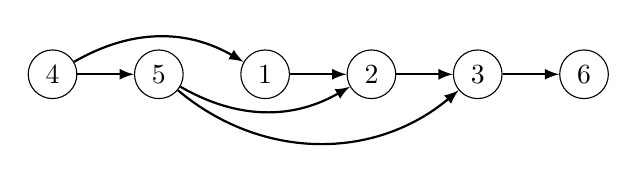
\begin{tikzpicture}[scale=0.9]
\node[draw, circle] (1) at (3,0) {$1$};
\node[draw, circle] (2) at (4.5,0) {$2$};
\node[draw, circle] (3) at (6,0) {$3$};
\node[draw, circle] (4) at (0,0) {$4$};
\node[draw, circle] (5) at (1.5,0) {$5$};
\node[draw, circle] (6) at (7.5,0) {$6$};

\path[draw,thick,->,>=latex] (1) -- (2);
\path[draw,thick,->,>=latex] (2) -- (3);
\path[draw,thick,->,>=latex] (4) edge [bend left=30] (1);
\path[draw,thick,->,>=latex] (4) -- (5);
\path[draw,thick,->,>=latex] (5) edge [bend right=30] (2);
\path[draw,thick,->,>=latex] (5) edge [bend right=40] (3);
\path[draw,thick,->,>=latex] (3) -- (6);
\end{tikzpicture}
\end{center}

Lưu ý rằng một sắp xếp tô pô không phải là duy nhất,
và có thể có nhiều cách sắp xếp tô pô cho một đồ thị.

\subsubsection{Ví dụ 2}

Bây giờ chúng ta hãy xem xét một đồ thị mà chúng ta
không thể xây dựng một sắp xếp tô pô,
bởi vì đồ thị chứa một chu trình:

\begin{center}
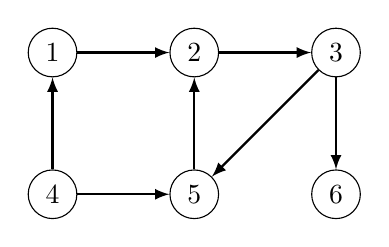
\begin{tikzpicture}[scale=0.9]
\node[draw, circle] (1) at (1,5) {$1$};
\node[draw, circle] (2) at (3,5) {$2$};
\node[draw, circle] (3) at (5,5) {$3$};
\node[draw, circle] (4) at (1,3) {$4$};
\node[draw, circle] (5) at (3,3) {$5$};
\node[draw, circle] (6) at (5,3) {$6$};

\path[draw,thick,->,>=latex] (1) -- (2);
\path[draw,thick,->,>=latex] (2) -- (3);
\path[draw,thick,->,>=latex] (4) -- (1);
\path[draw,thick,->,>=latex] (4) -- (5);
\path[draw,thick,->,>=latex] (5) -- (2);
\path[draw,thick,->,>=latex] (3) -- (5);
\path[draw,thick,->,>=latex] (3) -- (6);
\end{tikzpicture}
\end{center}
Việc tìm kiếm tiến hành như sau:
\begin{center}
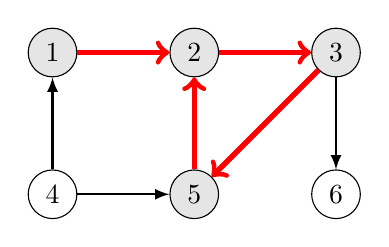
\begin{tikzpicture}[scale=0.9]
\node[draw, circle,fill=gray!20] (1) at (1,5) {$1$};
\node[draw, circle,fill=gray!20] (2) at (3,5) {$2$};
\node[draw, circle,fill=gray!20] (3) at (5,5) {$3$};
\node[draw, circle] (4) at (1,3) {$4$};
\node[draw, circle,fill=gray!20] (5) at (3,3) {$5$};
\node[draw, circle] (6) at (5,3) {$6$};

\path[draw,thick,->,>=latex] (4) -- (1);
\path[draw,thick,->,>=latex] (4) -- (5);
\path[draw,thick,->,>=latex] (3) -- (6);

\path[draw=red,thick,->,line width=2pt] (1) -- (2);
\path[draw=red,thick,->,line width=2pt] (2) -- (3);
\path[draw=red,thick,->,line width=2pt] (3) -- (5);
\path[draw=red,thick,->,line width=2pt] (5) -- (2);
\end{tikzpicture}
\end{center}
Việc tìm kiếm đến nút 2 có trạng thái là 1,
điều này có nghĩa là đồ thị chứa một chu trình.
Trong ví dụ này, có một chu trình
$2 \rightarrow 3 \rightarrow 5 \rightarrow 2$.

\section{Quy hoạch động (Dynamic programming)}

Nếu một đồ thị có hướng là không có chu trình,
quy hoạch động có thể được áp dụng cho nó.
Ví dụ, chúng ta có thể giải quyết hiệu quả các
vấn đề sau liên quan đến các đường đi từ một nút bắt đầu
đến một nút kết thúc:

\begin{itemize}
\item có bao nhiêu đường đi khác nhau?
\item đường đi ngắn nhất/dài nhất là gì?
\item số cạnh tối thiểu/tối đa trong một đường đi là bao nhiêu?
\item nút nào chắc chắn xuất hiện trong bất kỳ đường đi nào?
\end{itemize}

\subsubsection{Đếm số lượng đường đi}

Ví dụ, chúng ta hãy tính số lượng đường đi
từ nút 1 đến nút 6 trong đồ thị sau:

\begin{center}
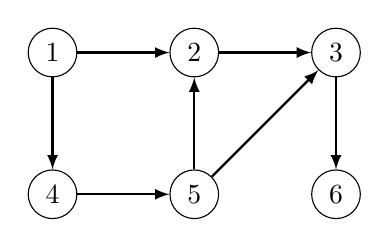
\begin{tikzpicture}[scale=0.9]
\node[draw, circle] (1) at (1,5) {$1$};
\node[draw, circle] (2) at (3,5) {$2$};
\node[draw, circle] (3) at (5,5) {$3$};
\node[draw, circle] (4) at (1,3) {$4$};
\node[draw, circle] (5) at (3,3) {$5$};
\node[draw, circle] (6) at (5,3) {$6$};

\path[draw,thick,->,>=latex] (1) -- (2);
\path[draw,thick,->,>=latex] (2) -- (3);
\path[draw,thick,->,>=latex] (1) -- (4);
\path[draw,thick,->,>=latex] (4) -- (5);
\path[draw,thick,->,>=latex] (5) -- (2);
\path[draw,thick,->,>=latex] (5) -- (3);
\path[draw,thick,->,>=latex] (3) -- (6);
\end{tikzpicture}
\end{center}
Có tổng cộng ba đường đi như vậy:
\begin{itemize}
\item $1 \rightarrow 2 \rightarrow 3 \rightarrow 6$
\item $1 \rightarrow 4 \rightarrow 5 \rightarrow 2 \rightarrow 3 \rightarrow 6$
\item $1 \rightarrow 4 \rightarrow 5 \rightarrow 3 \rightarrow 6$
\end{itemize}

Gọi $\texttt{paths}(x)$ là số lượng đường đi từ
nút 1 đến nút $x$.
Là trường hợp cơ sở, $\texttt{paths}(1)=1$.
Sau đó, để tính các giá trị khác của $\texttt{paths}(x)$,
chúng ta có thể sử dụng công thức đệ quy
\[\texttt{paths}(x) = \texttt{paths}(a_1)+\texttt{paths}(a_2)+\cdots+\texttt{paths}(a_k)\]
trong đó $a_1,a_2,\ldots,a_k$ là các nút mà từ đó có
một cạnh đến $x$.
Vì đồ thị không có chu trình, các giá trị của $\texttt{paths}(x)$
có thể được tính theo thứ tự của một sắp xếp tô pô.
Một sắp xếp tô pô cho đồ thị trên như sau:
\begin{center}
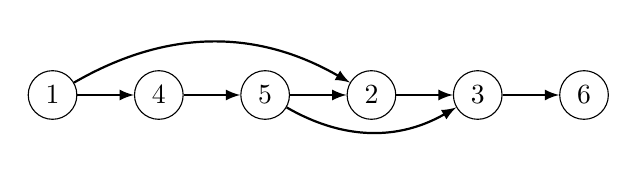
\begin{tikzpicture}[scale=0.9]
\node[draw, circle] (1) at (0,0) {$1$};
\node[draw, circle] (2) at (4.5,0) {$2$};
\node[draw, circle] (3) at (6,0) {$3$};
\node[draw, circle] (4) at (1.5,0) {$4$};
\node[draw, circle] (5) at (3,0) {$5$};
\node[draw, circle] (6) at (7.5,0) {$6$};

\path[draw,thick,->,>=latex] (1) edge [bend left=30] (2);
\path[draw,thick,->,>=latex] (2) -- (3);
\path[draw,thick,->,>=latex] (1) -- (4);
\path[draw,thick,->,>=latex] (4) -- (5);
\path[draw,thick,->,>=latex] (5) -- (2);
\path[draw,thick,->,>=latex] (5) edge [bend right=30] (3);
\path[draw,thick,->,>=latex] (3) -- (6);
\end{tikzpicture}
\end{center}
Do đó, số lượng đường đi như sau:
\begin{center}
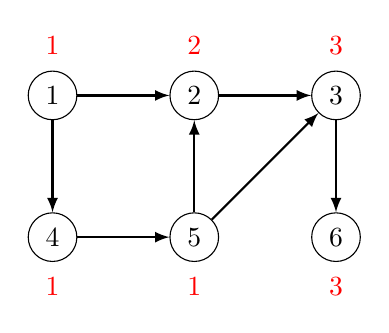
\begin{tikzpicture}[scale=0.9]
\node[draw, circle] (1) at (1,5) {$1$};
\node[draw, circle] (2) at (3,5) {$2$};
\node[draw, circle] (3) at (5,5) {$3$};
\node[draw, circle] (4) at (1,3) {$4$};
\node[draw, circle] (5) at (3,3) {$5$};
\node[draw, circle] (6) at (5,3) {$6$};

\path[draw,thick,->,>=latex] (1) -- (2);
\path[draw,thick,->,>=latex] (2) -- (3);
\path[draw,thick,->,>=latex] (1) -- (4);
\path[draw,thick,->,>=latex] (4) -- (5);
\path[draw,thick,->,>=latex] (5) -- (2);
\path[draw,thick,->,>=latex] (5) -- (3);
\path[draw,thick,->,>=latex] (3) -- (6);

\node[color=red] at (1,2.3) {$1$};
\node[color=red] at (3,2.3) {$1$};
\node[color=red] at (5,2.3) {$3$};
\node[color=red] at (1,5.7) {$1$};
\node[color=red] at (3,5.7) {$2$};
\node[color=red] at (5,5.7) {$3$};
\end{tikzpicture}
\end{center}

Ví dụ, để tính giá trị của $\texttt{paths}(3)$,
chúng ta có thể sử dụng công thức $\texttt{paths}(2)+\texttt{paths}(5)$,
bởi vì có các cạnh từ các nút 2 và 5
đến nút 3.
Vì $\texttt{paths}(2)=2$ và $\texttt{paths}(5)=1$, chúng ta kết luận rằng $\texttt{paths}(3)=3$.

\subsubsection{Mở rộng thuật toán Dijkstra}

\index{Dijkstra's algorithm}

Một sản phẩm phụ của thuật toán Dijkstra là một đồ thị có hướng, không chu trình
chỉ ra cho mỗi nút của đồ thị ban đầu
các cách khả dĩ để đến nút đó bằng một đường đi ngắn nhất
từ nút bắt đầu.
Quy hoạch động có thể được áp dụng cho đồ thị đó.
Ví dụ, trong đồ thị
\begin{center}
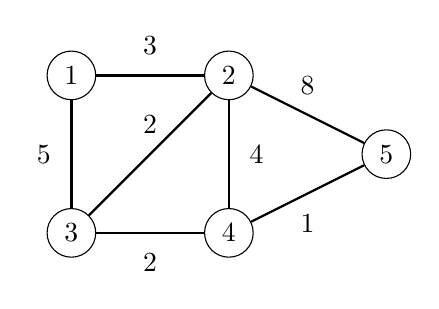
\begin{tikzpicture}
\node[draw, circle] (1) at (0,0) {$1$};
\node[draw, circle] (2) at (2,0) {$2$};
\node[draw, circle] (3) at (0,-2) {$3$};
\node[draw, circle] (4) at (2,-2) {$4$};
\node[draw, circle] (5) at (4,-1) {$5$};

\path[draw,thick,-] (1) -- node[font=\small,label=above:3] {} (2);
\path[draw,thick,-] (1) -- node[font=\small,label=left:5] {} (3);
\path[draw,thick,-] (2) -- node[font=\small,label=right:4] {} (4);
\path[draw,thick,-] (2) -- node[font=\small,label=above:8] {} (5);
\path[draw,thick,-] (3) -- node[font=\small,label=below:2] {} (4);
\path[draw,thick,-] (4) -- node[font=\small,label=below:1] {} (5);
\path[draw,thick,-] (2) -- node[font=\small,label=above:2] {} (3);
\end{tikzpicture}
\end{center}
các đường đi ngắn nhất từ nút 1 có thể sử dụng các cạnh sau:
\begin{center}
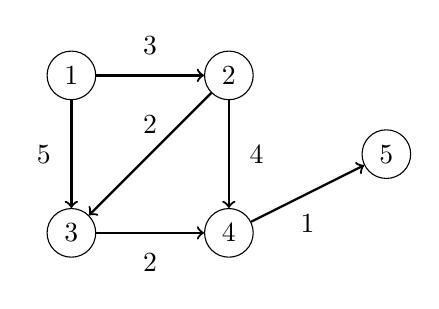
\begin{tikzpicture}
\node[draw, circle] (1) at (0,0) {$1$};
\node[draw, circle] (2) at (2,0) {$2$};
\node[draw, circle] (3) at (0,-2) {$3$};
\node[draw, circle] (4) at (2,-2) {$4$};
\node[draw, circle] (5) at (4,-1) {$5$};

\path[draw,thick,->] (1) -- node[font=\small,label=above:3] {} (2);
\path[draw,thick,->] (1) -- node[font=\small,label=left:5] {} (3);
\path[draw,thick,->] (2) -- node[font=\small,label=right:4] {} (4);
\path[draw,thick,->] (3) -- node[font=\small,label=below:2] {} (4);
\path[draw,thick,->] (4) -- node[font=\small,label=below:1] {} (5);
\path[draw,thick,->] (2) -- node[font=\small,label=above:2] {} (3);
\end{tikzpicture}
\end{center}

Bây giờ chúng ta có thể, ví dụ, tính số lượng
đường đi ngắn nhất từ nút 1 đến nút 5
sử dụng quy hoạch động:
\begin{center}
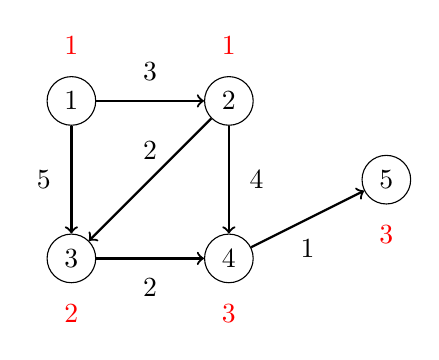
\begin{tikzpicture}
\node[draw, circle] (1) at (0,0) {$1$};
\node[draw, circle] (2) at (2,0) {$2$};
\node[draw, circle] (3) at (0,-2) {$3$};
\node[draw, circle] (4) at (2,-2) {$4$};
\node[draw, circle] (5) at (4,-1) {$5$};

\path[draw,thick,->] (1) -- node[font=\small,label=above:3] {} (2);
\path[draw,thick,->] (1) -- node[font=\small,label=left:5] {} (3);
\path[draw,thick,->] (2) -- node[font=\small,label=right:4] {} (4);
\path[draw,thick,->] (3) -- node[font=\small,label=below:2] {} (4);
\path[draw,thick,->] (4) -- node[font=\small,label=below:1] {} (5);
\path[draw,thick,->] (2) -- node[font=\small,label=above:2] {} (3);

\node[color=red] at (0,0.7) {$1$};
\node[color=red] at (2,0.7) {$1$};
\node[color=red] at (0,-2.7) {$2$};
\node[color=red] at (2,-2.7) {$3$};
\node[color=red] at (4,-1.7) {$3$};
\end{tikzpicture}
\end{center}

\subsubsection{Biểu diễn bài toán dưới dạng đồ thị}

Thực ra, bất kỳ bài toán quy hoạch động nào
cũng có thể được biểu diễn dưới dạng một đồ thị có hướng, không chu trình.
Trong một đồ thị như vậy, mỗi nút tương ứng với một trạng thái quy hoạch động
và các cạnh chỉ ra cách các trạng thái phụ thuộc vào nhau.

Ví dụ, xem xét bài toán
tạo thành một tổng tiền $n$
sử dụng các đồng xu
$\{c_1,c_2,\ldots,c_k\}$.
Trong bài toán này, chúng ta có thể xây dựng một đồ thị trong đó
mỗi nút tương ứng với một tổng tiền,
và các cạnh cho thấy cách các đồng xu có thể được chọn.
Ví dụ, đối với các đồng xu $\{1,3,4\}$ và $n=6$,
đồ thị như sau:
\begin{center}
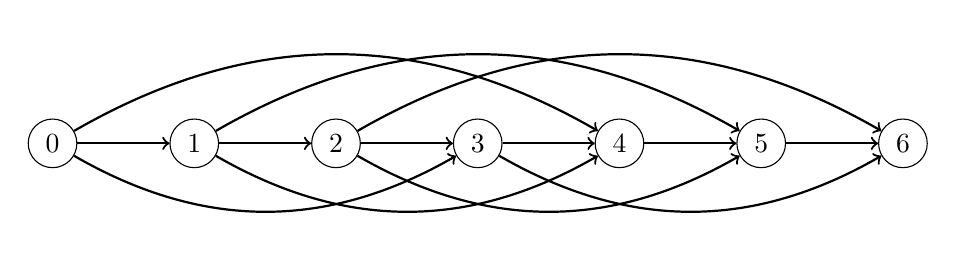
\begin{tikzpicture}[scale=0.9]
\node[draw, circle] (0) at (0,0) {$0$};
\node[draw, circle] (1) at (2,0) {$1$};
\node[draw, circle] (2) at (4,0) {$2$};
\node[draw, circle] (3) at (6,0) {$3$};
\node[draw, circle] (4) at (8,0) {$4$};
\node[draw, circle] (5) at (10,0) {$5$};
\node[draw, circle] (6) at (12,0) {$6$};

\path[draw,thick,->] (0) -- (1);
\path[draw,thick,->] (1) -- (2);
\path[draw,thick,->] (2) -- (3);
\path[draw,thick,->] (3) -- (4);
\path[draw,thick,->] (4) -- (5);
\path[draw,thick,->] (5) -- (6);

\path[draw,thick,->] (0) edge [bend right=30] (3);
\path[draw,thick,->] (1) edge [bend right=30] (4);
\path[draw,thick,->] (2) edge [bend right=30] (5);
\path[draw,thick,->] (3) edge [bend right=30] (6);

\path[draw,thick,->] (0) edge [bend left=30] (4);
\path[draw,thick,->] (1) edge [bend left=30] (5);
\path[draw,thick,->] (2) edge [bend left=30] (6);
\end{tikzpicture}
\end{center}

Sử dụng biểu diễn này,
đường đi ngắn nhất từ nút 0 đến nút $n$
tương ứng với một giải pháp với số lượng đồng xu tối thiểu,
và tổng số đường đi từ nút 0 đến nút $n$
bằng tổng số lời giải.

\section{Đường đi kế tiếp}

\index{đồ thị kế tiếp}
\index{đồ thị hàm}

Trong phần còn lại của chương,
chúng ta sẽ tập trung vào \key{đồ thị kế tiếp (successor graphs)}.
Trong các đồ thị đó,
bán bậc ngoài của mỗi nút là 1, tức là,
chính xác một cạnh bắt đầu tại mỗi nút.
Một đồ thị kế tiếp bao gồm một hoặc nhiều
thành phần, mỗi thành phần chứa
một chu trình và một số đường đi dẫn đến nó.

Đồ thị kế tiếp đôi khi được gọi là
\key{đồ thị hàm (functional graphs)}.
Lý do cho điều này là bất kỳ đồ thị kế tiếp nào
cũng tương ứng với một hàm xác định
các cạnh của đồ thị.
Tham số cho hàm là một nút của đồ thị,
và hàm trả về nút kế tiếp của nút đó.

Ví dụ, hàm
\begin{center}
\begin{tabular}{r|rrrrrrrrr}
$x$ & 1 & 2 & 3 & 4 & 5 & 6 & 7 & 8 & 9 \\
\hline
$\texttt{succ}(x)$ & 3 & 5 & 7 & 6 & 2 & 2 & 1 & 6 & 3 \\
\end{tabular}
\end{center}
xác định đồ thị sau:
\begin{center}
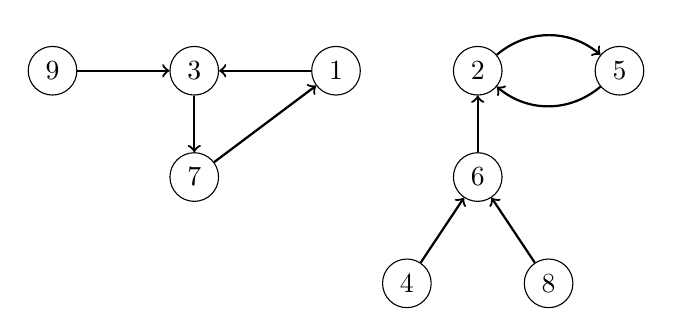
\begin{tikzpicture}[scale=0.9]
\node[draw, circle] (1) at (0,0) {$1$};
\node[draw, circle] (2) at (2,0) {$2$};
\node[draw, circle] (3) at (-2,0) {$3$};
\node[draw, circle] (4) at (1,-3) {$4$};
\node[draw, circle] (5) at (4,0) {$5$};
\node[draw, circle] (6) at (2,-1.5) {$6$};
\node[draw, circle] (7) at (-2,-1.5) {$7$};
\node[draw, circle] (8) at (3,-3) {$8$};
\node[draw, circle] (9) at (-4,0) {$9$};

\path[draw,thick,->] (1) -- (3);
\path[draw,thick,->] (2)  edge [bend left=40] (5);
\path[draw,thick,->] (3) -- (7);
\path[draw,thick,->] (4) -- (6);
\path[draw,thick,->] (5)  edge [bend left=40] (2);
\path[draw,thick,->] (6) -- (2);
\path[draw,thick,->] (7) -- (1);
\path[draw,thick,->] (8) -- (6);
\path[draw,thick,->] (9) -- (3);
\end{tikzpicture}
\end{center}

Vì mỗi nút của một đồ thị kế tiếp có một
nút kế tiếp duy nhất, chúng ta cũng có thể định nghĩa một hàm $\texttt{succ}(x,k)$
trả về nút mà chúng ta sẽ đến nếu
chúng ta bắt đầu tại nút $x$ và đi $k$ bước về phía trước.
Ví dụ, trong đồ thị trên $\texttt{succ}(4,6)=2$,
bởi vì chúng ta sẽ đến nút 2 bằng cách đi 6 bước từ nút 4:

\begin{center}
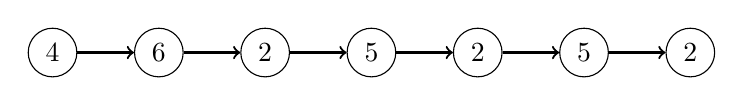
\begin{tikzpicture}[scale=0.9]
\node[draw, circle] (1) at (0,0) {$4$};
\node[draw, circle] (2) at (1.5,0) {$6$};
\node[draw, circle] (3) at (3,0) {$2$};
\node[draw, circle] (4) at (4.5,0) {$5$};
\node[draw, circle] (5) at (6,0) {$2$};
\node[draw, circle] (6) at (7.5,0) {$5$};
\node[draw, circle] (7) at (9,0) {$2$};

\path[draw,thick,->] (1) -- (2);
\path[draw,thick,->] (2) -- (3);
\path[draw,thick,->] (3) -- (4);
\path[draw,thick,->] (4) -- (5);
\path[draw,thick,->] (5) -- (6);
\path[draw,thick,->] (6) -- (7);
\end{tikzpicture}
\end{center}

Một cách đơn giản để tính một giá trị của $\texttt{succ}(x,k)$
là bắt đầu tại nút $x$ và đi $k$ bước về phía trước, mất thời gian $O(k)$.
Tuy nhiên, bằng cách sử dụng tiền xử lý, bất kỳ giá trị nào của $\texttt{succ}(x,k)$
cũng có thể được tính chỉ trong thời gian $O(\log k)$.

Ý tưởng là tính trước tất cả các giá trị của $\texttt{succ}(x,k)$ trong đó
$k$ là một lũy thừa của hai và tối đa là $u$, trong đó $u$ là
số bước tối đa chúng ta sẽ đi.
Điều này có thể được thực hiện hiệu quả, bởi vì
chúng ta có thể sử dụng công thức đệ quy sau:

\begin{equation*}
    \texttt{succ}(x,k) = \begin{cases}
               \texttt{succ}(x)              & k = 1\\
               \texttt{succ}(\texttt{succ}(x,k/2),k/2)   & k > 1\\
           \end{cases}
\end{equation*}

Việc tính toán trước các giá trị mất thời gian $O(n \log u)$,
bởi vì $O(\log u)$ giá trị được tính cho mỗi nút.
Trong đồ thị trên, các giá trị đầu tiên như sau:

\begin{center}
\begin{tabular}{r|rrrrrrrrr}
$x$ & 1 & 2 & 3 & 4 & 5 & 6 & 7 & 8 & 9 \\
\hline
$\texttt{succ}(x,1)$ & 3 & 5 & 7 & 6 & 2 & 2 & 1 & 6 & 3 \\
$\texttt{succ}(x,2)$ & 7 & 2 & 1 & 2 & 5 & 5 & 3 & 2 & 7 \\
$\texttt{succ}(x,4)$ & 3 & 2 & 7 & 2 & 5 & 5 & 1 & 2 & 3 \\
$\texttt{succ}(x,8)$ & 7 & 2 & 1 & 2 & 5 & 5 & 3 & 2 & 7 \\
$\cdots$ \\
\end{tabular}
\end{center}

Sau đó, bất kỳ giá trị nào của $\texttt{succ}(x,k)$ cũng có thể được tính toán
bằng cách biểu diễn số bước $k$ dưới dạng tổng các lũy thừa của hai.
Ví dụ, nếu chúng ta muốn tính giá trị của $\texttt{succ}(x,11)$,
chúng ta trước tiên tạo biểu diễn $11=8+2+1$.
Sử dụng điều đó,
\[\texttt{succ}(x,11)=\texttt{succ}(\texttt{succ}(\texttt{succ}(x,8),2),1).\]
Ví dụ, trong đồ thị trước đó
\[\texttt{succ}(4,11)=\texttt{succ}(\texttt{succ}(\texttt{succ}(4,8),2),1)=5.\]

Một biểu diễn như vậy luôn bao gồm
$O(\log k)$ phần, vì vậy việc tính một giá trị của $\texttt{succ}(x,k)$
mất thời gian $O(\log k)$.

\section{Dò tìm chu trình (Cycle detection)}

\index{chu trình}
\index{dò tìm chu trình}

Xem xét một đồ thị kế tiếp chỉ chứa
một đường đi kết thúc bằng một chu trình.
Chúng ta có thể đặt ra các câu hỏi sau:
nếu chúng ta bắt đầu đi từ nút xuất phát,
nút đầu tiên trong chu trình là gì
và chu trình chứa bao nhiêu nút?

Ví dụ, trong đồ thị

\begin{center}
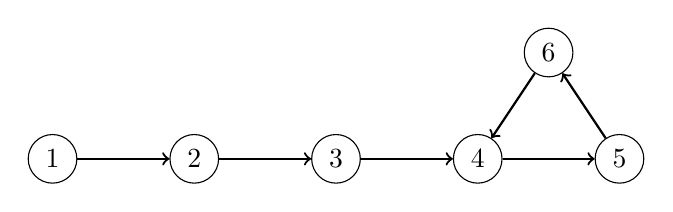
\begin{tikzpicture}[scale=0.9]
\node[draw, circle] (5) at (0,0) {$5$};
\node[draw, circle] (4) at (-2,0) {$4$};
\node[draw, circle] (6) at (-1,1.5) {$6$};
\node[draw, circle] (3) at (-4,0) {$3$};
\node[draw, circle] (2) at (-6,0) {$2$};
\node[draw, circle] (1) at (-8,0) {$1$};

\path[draw,thick,->] (1) -- (2);
\path[draw,thick,->] (2) -- (3);
\path[draw,thick,->] (3) -- (4);
\path[draw,thick,->] (4) -- (5);
\path[draw,thick,->] (5) -- (6);
\path[draw,thick,->] (6) -- (4);
\end{tikzpicture}
\end{center}
chúng ta bắt đầu đi tại nút 1,
nút đầu tiên thuộc về chu trình là nút 4, và chu trình bao gồm
ba nút (4, 5 và 6).

Một cách đơn giản để phát hiện chu trình là đi trong
đồ thị và theo dõi
tất cả các nút đã được thăm. Một khi một nút được thăm
lần thứ hai, chúng ta có thể kết luận
rằng nút đó là nút đầu tiên trong chu trình.
Phương pháp này hoạt động trong thời gian $O(n)$ và cũng sử dụng
bộ nhớ $O(n)$.

Tuy nhiên, có những thuật toán tốt hơn để dò tìm chu trình.
Độ phức tạp thời gian của các thuật toán như vậy vẫn là $O(n)$,
nhưng chúng chỉ sử dụng bộ nhớ $O(1)$.
Đây là một cải tiến quan trọng nếu $n$ lớn.
Tiếp theo chúng ta sẽ thảo luận về thuật toán Floyd
đạt được các thuộc tính này.

\subsubsection{Thuật toán Floyd}

\index{Floyd's algorithm}

\key{Thuật toán Floyd (Floyd's algorithm)}\footnote{Ý tưởng của thuật toán được đề cập trong \cite{knu982}
và được cho là của R. W. Floyd; tuy nhiên, không rõ liệu Floyd có thực sự
phát hiện ra thuật toán này hay không.} đi về phía trước
trong đồ thị bằng cách sử dụng hai con trỏ $a$ và $b$.
Cả hai con trỏ đều bắt đầu tại một nút $x$
là nút xuất phát của đồ thị.
Sau đó, ở mỗi lượt, con trỏ $a$ đi
một bước về phía trước và con trỏ $b$
đi hai bước về phía trước.
Quá trình tiếp tục cho đến khi
các con trỏ gặp nhau:
\begin{lstlisting}
a = succ(x);
b = succ(succ(x));
while (a != b) {
    a = succ(a);
    b = succ(succ(b));
}
\end{lstlisting}

Tại thời điểm này, con trỏ $a$ đã đi được $k$ bước
và con trỏ $b$ đã đi được $2k$ bước,
vì vậy độ dài của chu trình là ước của $k$.
Do đó, nút đầu tiên thuộc về chu trình
có thể được tìm thấy bằng cách di chuyển con trỏ $a$ đến nút $x$
và tiến các con trỏ
từng bước một cho đến khi chúng gặp lại nhau.
\begin{lstlisting}
a = x;
while (a != b) {
    a = succ(a);
    b = succ(b);
}
first = a; // nut dau tien
\end{lstlisting}

Sau đó, độ dài của chu trình
có thể được tính như sau:
\begin{lstlisting}
b = succ(a);
length = 1; // do dai
while (a != b) {
    b = succ(b);
    length++;
}
\end{lstlisting}